
\begin{frame}{Trykjagt (bewegungsjagt)}
    
    \begin{columns}[T]
        \begin{column}{0.58\textwidth}
            \begin{itemize}
                \item Semi-aktiv jagtform med få drivere 
                \item Jægere placeres vilkårligt i terræn
                \item Få drivere skubber rundt til hovdyr
                \item Der anvendes riffel eller bue
                \item Der anvendes sjældent hunde i så fald meget kortsøgende eller i snor
                \item Dyrene kommer langsomt (=bedre skydning/afskydning))
                \item Jægere er typisk placeret i stiger, tårne eller treestand
            \end{itemize}
        \end{column}
        
        \begin{column}{0.4\textwidth}
            \centering
            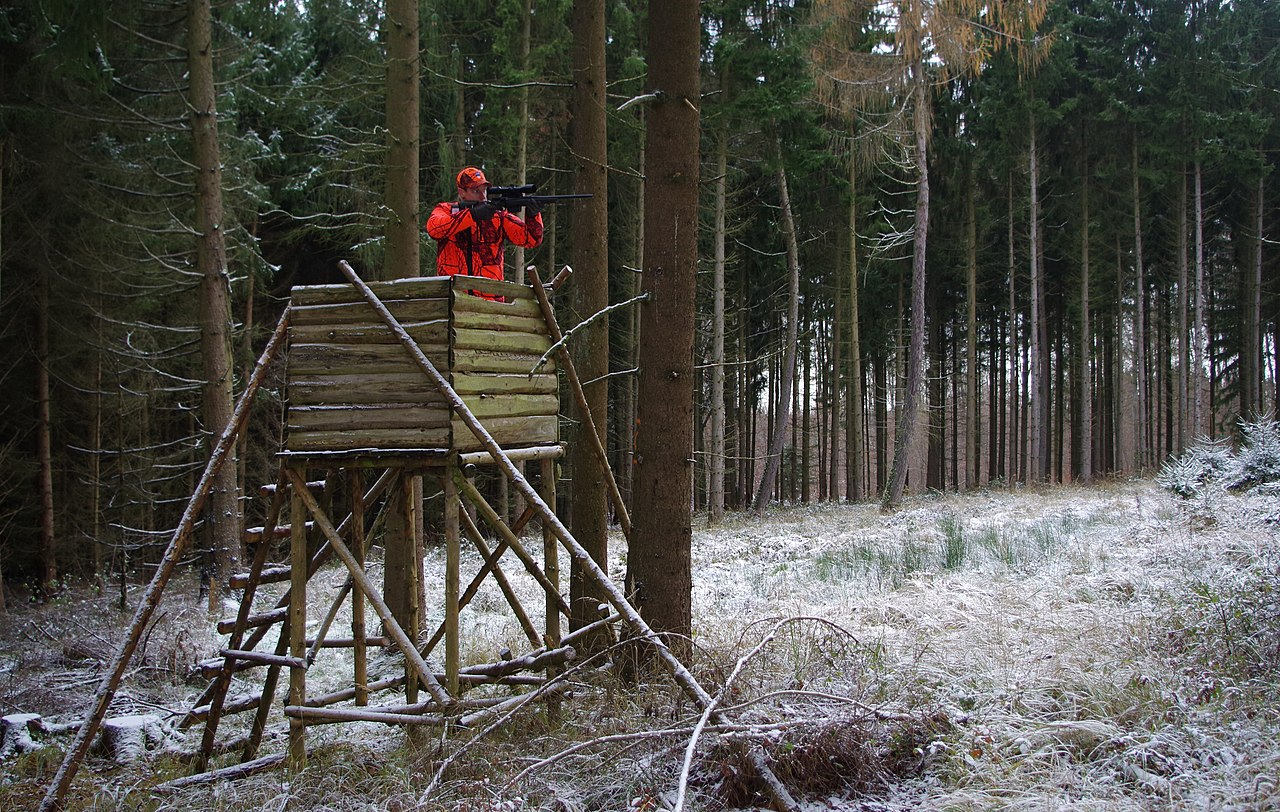
\includegraphics[width=\textwidth,height=0.85\textheight,keepaspectratio]
                {Billeder/Jagtformer/trykjagt_01}
            % Alternativt brug en af disse stilrene billeder:
            % \includegraphics[width=\textwidth]{highseat-snow-forest-hunter.jpg}
            % \includegraphics[width=\textwidth]{hunter-leaning-tree-rifle.jpg}
        \end{column}
    \end{columns}
    
\end{frame}